\documentclass[10pt, compress, usenames, dvipsnames]{beamer}

\usetheme{m}
\usepackage{booktabs}
\usepackage[scale=2]{ccicons}
\usepackage{minted}
\usepackage{listings}
\usepackage{scrextend}

% set the default code style
\lstset{
    frame=tb, % draw a frame at the top and bottom of the code block
    tabsize=4, % tab space width
    showstringspaces=false, % don't mark spaces in strings
    numbers=left, % display line numbers on the left
    commentstyle=\color{OliveGreen}, % comment color
    keywordstyle=\color{MidnightBlue}, % keyword color
    stringstyle=\color{WildStrawberry}, % string color
	language=C++,
	basicstyle=\ttfamily
}

\usemintedstyle{trac}


\begin{document}

\title{Polymorphism}
\subtitle{Object behavior in different contexts}
\date{\today}
\author{Florian Warg, Max Staff}

\maketitle

\begin{frame}[fragile]
    \frametitle{What is polymorphism?}
    \begin{itemize}
    \item polymorphism is the ability of an object to take on many forms
    \item if an object passes more than 1 "is-a" tests, it is considered polymorphic
    \item i.e. if a class is derived from another class, its objects are polymorphic
    \item 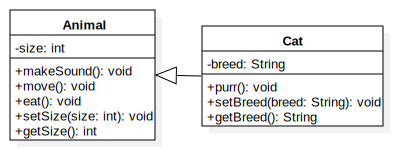
\includegraphics{img/polymorph-animal-cat}    
    \item objects of "Cat" are polymorphic because they are of type "Cat" and "Animal"
    \end{itemize}
\end{frame}

\begin{frame}[fragile]
    \frametitle{Polymorphism in C++}
    \begin{itemize}
    \item polymorphism only works with reference types (in all languages)
    \begin{lstlisting}[numbers=none]
Cat felix;
felix.purr();
Animal& alsoFelix = felix;
alsoFelix.purr(); // error
felix.getSize();  // OK
    \end{lstlisting}
    \item felix is a cat and also an animal
    \item i.e. felix is polymorphic
    \item we can treat felix as a generic animal instead of a cat by using references or pointers
    \item now only the "animal" interface is exposed
    \end{itemize}
\end{frame}

\begin{frame}[fragile]
    \frametitle{Implicit reference casts}
    \begin{itemize}
    \item the compiler can implicitly cast a reference to a parent-type reference
    \item this allows functions to accept multiple types
    \begin{lstlisting}[numbers=none]
void printSize(const Animal& animal) {
    cout << animal.getSize();
}
Cat felix;
printSize(felix); // OK
    \end{lstlisting}
    \end{itemize}
\end{frame}

\begin{frame}[fragile]
    \frametitle{Different behavior}
    \begin{itemize}
    \item what happens when Cat has a method with the same name
    \begin{lstlisting}[numbers=none]
class Animal {
public:
    void makeSound() { 
        cout << "Animal::makeSound()\n"; }
};
class Cat : public Animal {
public:
    void makeSound() {
        cout << "Cat::makeSound()\n"; }
};
Cat felix;
Animal& alsoFelix = felix;
felix.makeSound();     // Cat::makeSound()
alsoFelix.makeSound(); // Animal::makeSound()
    \end{lstlisting}
    \end{itemize}
\end{frame}

\begin{frame}[fragile]
    \frametitle{Overriding methods}
    \begin{itemize}
    \item a child class can override a method of its parent
    \item a method is overridable if it is virtual
    \item use \lstinline{override} keyword for compiler checks
    \begin{lstlisting}[numbers=none]
class Animal {
public:
    virtual void makeSound();
};
class Cat : public Animal {
public:
    void makeSound() override {
        cout << "Cat::makeSound()\n"; }
};
Cat felix;
Animal& alsoFelix = felix;
felix.makeSound();     // Cat::makeSound()
alsoFelix.makeSound(); // Cat::makeSound()
    \end{lstlisting}
    \end{itemize}
\end{frame}

\begin{frame}[fragile]
    \frametitle{Lifetime of basic objects}
    \begin{itemize}
    \begin{lstlisting}[numbers=none]
struct A {
    int i;
    string str;
};
    \end{lstlisting}
    \item construct i
    \item construct str
    \item call \lstinline{A()}
    \item call \lstinline{~A()}
    \item destruct str
    \item destruct i
    \end{itemize}
\end{frame}

\begin{frame}[fragile]
    \frametitle{Lifetime with inheritance}
    \begin{itemize}
    \begin{lstlisting}[numbers=none]
struct A { /* ... */ };
struct B : public A {
    int i;
    string str;
};
    \end{lstlisting}
    \item construct A
    \item construct i
    \item construct str
    \item call \lstinline{B()}
    \item call \lstinline{~B()}
    \item destruct str
    \item destruct i
    \item destruct A
    \end{itemize}
\end{frame}

\begin{frame}[fragile]
    \frametitle{new and delete}
    \begin{itemize}
    \item consider this primitive implementation of a delete function
    \begin{lstlisting}[numbers=none]
delete(T* ptr) {
    ptr->~T();
    free(ptr);
}
class Parent {};
class Child : public Parent {};
Parent* p = new Child();
delete(p); // what happens here?
    \end{lstlisting}
    \item our defined delete function behaves like the real keyword
    \item since p points to a Parent object, only the parent dtor is invoked
    \item we already know how to fix this (-> virtual functions)
    \end{itemize}
\end{frame}

\begin{frame}[fragile]
    \frametitle{No more implicit memory leaks}
    \begin{itemize}
    \begin{lstlisting}[numbers=none]
class Parent {
public:
    virtual ~Parent() = default;
};
class Child : public Parent {};
Parent* p = new Child();
delete p;
    \end{lstlisting}
    \item now the child dtor overrides the parent dtor
    \item make sure to have a virtual destructor if you want to derive from a class
    \item introducing virtual functions comes with an overhead
    \item each class needs a vtable, objects need a vtable pointer
    \item when calling functions, virtual dispatch is needed
    \end{itemize}
\end{frame}

\end{document}
